\documentclass[12pt,letterpaper]{article}
\usepackage{fullpage, times}
\usepackage{ctable}
\begin{document}
\title{Deploying and Sharing QSAR Models using Predictive Model Markup Language}
\author{Villu Ruusmann${}^{\dagger}$ and Rajarshi Guha${}^{\ddagger}$\\
${}^{\ddagger}$National Center for Advancing Translational Sciences\\ 9800 Medical Center Drive  Rockville, MD 20850 \\ \\
${}^{\dagger}$Your address }
\date{}
\maketitle
\begin{abstract}
  A nice abstract
\end{abstract}

\section{A Plethora of Predictive Models}
\label{sec:introduction}

Quantitative Structure-Activity Relationship (QSAR) models have become
ubiquitous in computational chemistry and cheminformatics, having been
built for a variety of endpoints including biological activities and
physical properties. As shown in Figure \ref{fig:count-qsar} the last
15 years has seen a significant increase in publications developing or
using QSAR models. While there has been much discussion (REFS) on the
prospective utility and validity of predictive QSAR models, a key
bottleneck to their assessment is the fact that they are not easily
obtainable. That is, the bulk of QSAR models are described in a
publication in terms of the descriptors (sometimes made available) and
the modeling method. While the implementation is noted, it is upon the
reader to actually obtain the descriptor values, obtain and set up the
modeling environment and then actually rebuild the model. In other
words, the actual model that was developed by the authors is, usually,
not available to be used directly. In a few cases, the model may be
built in a pipeline tool [REF], which alleviates this problem to some
extent. Furthermore, the model development workflow usually involves
multiple software tools, each one of a specific version. Without
access to the exact same version of these tools, a user cannot be
guaranteed to exactly reproduce the model that the authors
describe. The issue of reproducibility (of workflows and results) has
become increasingly important [REF Greg Landrum] in the computational
arena.

A number of workers have described infrastructure to deploy predictive
models. Some platforms such as Pipeline Pilot provide a easy to use
method to deploy a complete pipeline as a web page. However, this
approach does not allow one to share models with users who do not have
access to the software. Guha [REF] described a web based
infrastructure that allowed one to deploy serialized models developed
in R. This architecture allowed one to distribute the model via a web
page, allowing users to provide new input and retrieve
predictions. But by virtue of using serialized R models, it allowed
the user to directly work with the original model itself. An important
downside was that the model itself did not contain explicit references
to the descriptors that were required as input. 


\ctable[cap={}, caption={Growth in number of Pubmed articles that use the term QSAR.},
label={fig:count-qsar},figure,botcap]
{c}
{}
{
  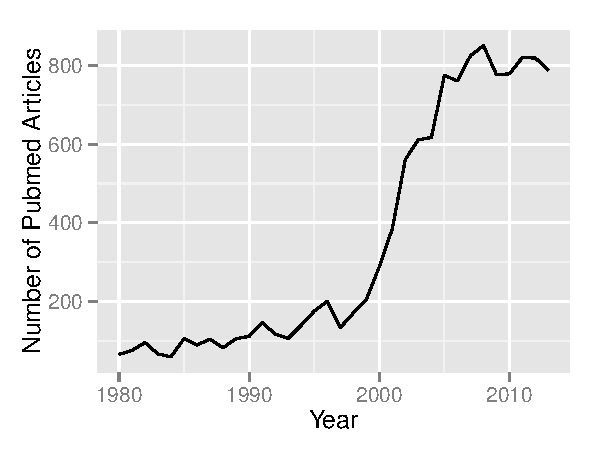
\includegraphics{img/count-qsar}
}

\section{Methods}
\label{sec:methods}

\subsection{Model Development}
\label{sec:model-development}


\subsection{Model Deployment}
\label{sec:model-deployment}


\section{Discussion}
\label{sec:discussion}



\end{document}
